% chapter 2

\chapter{相关技术理论}

\section{引言}
设计中的两个翻译技术均由深度学习的模型训练得出,本章具体介绍图片翻译文本技术和文本翻译图片技术的前置理论。

图片翻译文本技术的主体使用了编码-解码架构的长短期记忆模型。长短期记忆模型是一种特殊的循环神经网络,接下来首先将详细介绍神经网络、循环神经网络、长短期记忆的原理和模型结构,并阐述长短期记忆适用于文本生成的援引。文本翻译图片技术的主体使用了GAN网络模型。由于GAN网络模型在图片生成的领域内已经有了几个大的突破,我将在介绍GAN模型的结构和原理后,介绍相关的GAN模型的分支优化算法在图片生成领域的表现。

\section{图片翻译文本相关工作}
本次设计中图片字幕技术部分主要使用的技术基于长短期记忆循环神经网络。这一小节将阐述循环神经网络和长短期记忆的相关技术。
\subsection{神经网络}
神经网络(Neural Networks)是近年比较流行的概念。在2006年Hiinton\upcite{hinton2006reducing}提出深度学习概念后,成为了优化算法表现性能的一大利器。

神经网络的基本结构就是由神经元构成的网络,每个神经元结构如图~\ref{fig:nnc}所示,输入输出关系如式\eqref{eq:nn}表述结果。
\begin{equation}
    \label{eq:nn}
    f( \sum\limits_{i=1}^{m} w_i x_i + b ) 
\end{equation}
其中,$w$是神经网络上的边权(weight),$x$代表着输入数据,$b$则是神经网络中神经元的偏差值(bias)。

对于第$j$层的每一个神经元,它会对上一层的每一个神经元输入的$x_i$赋予权重$w_i$,计算出输出结果,即如式\eqref{eq:nnj}所示,其中n是每一层的神经元个数,由输入神经元个数决定。
\begin{equation}
    \label{eq:nnj}
    x_k^j = \sum\limits_{i=1}^{n} w_ik x_ik, k\in \left[1,n\right]
\end{equation}

\begin{figure}[b]
    \centering
    \begin{minipage}[t]{0.4\linewidth}
        \centering
        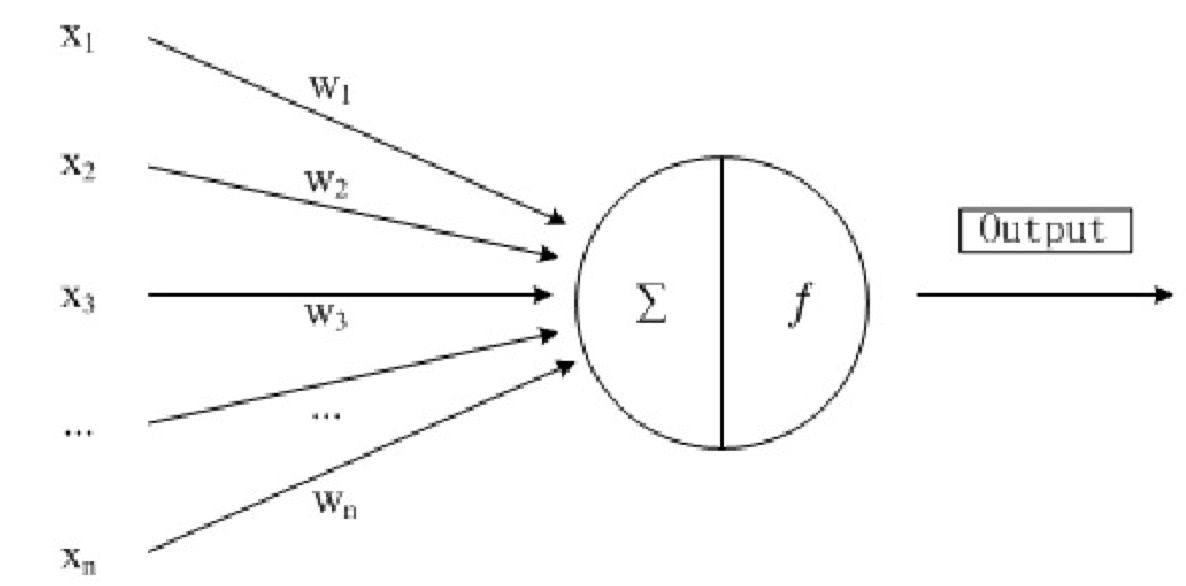
\includegraphics[width=0.9\textwidth]
        {figures/nnc.png}\\
        \caption{神经网络神经元}
        \label{fig:nnc}
    \end{minipage}
    \begin{minipage}[t]{0.5\linewidth}
        \centering
        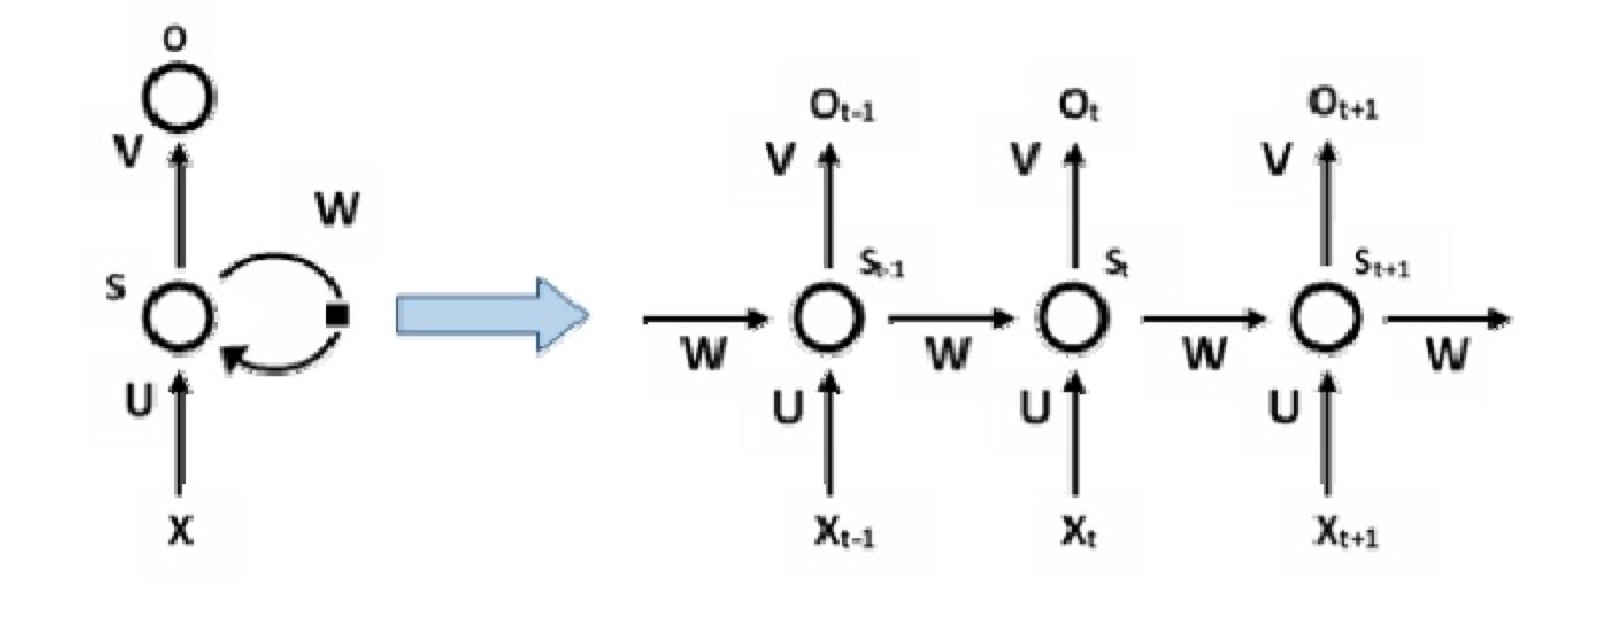
\includegraphics[width=0.9\textwidth]
        {figures/rnnc.png}\\
        \caption{循环神经网络神经元}
        \label{fig:rnnc}
    \end{minipage}
\end{figure}

\subsection{循环神经网络}
循环神经网络(Recurrent Neural Networks, RNN)是一种特殊的神经网络。为了加强上文信息对当前节点的影响,循环神经网络对神经元的输入数据增加了上一时序同一神经元的输出数据。它被广泛地运用在图像处理和自然语言处理上。与一般的神经网络相同,它也有前馈层和反馈层,但是它在一般的神经网络基础上增加了基于时序的循环机制。在一般的神经网络中,神经元之间相互独立,但是现实中的信息往往互相关联。所以,循环神经网络的特点像人一样有记忆的能力它的输出不仅依靠当前输入,也依靠历史的输出。在一定程度上,它更能反应真实的情况。

RNN神经元的结构与BP神经网络神经元有些许不同。如图~\ref{fig:rnnc}所示,任一隐藏层中神经元的输出信息依靠当前时刻的输入信息和前序时序的输出信息决定,同时当前时序的输出信息也会作为下一个神经元的输入。这样的神经网络构建了神经元之间的联系,让数据有了更为有效的依赖关系,优化了信息利用的效率。
每一个神经元的计算方式可以表述为式\eqref{eq:rnn}。其中$x_t$代表$t$时刻神经元的输入,$s_t$代表$t$时刻神经元的状态,$o_t$代表$t$时刻神经元的输出。
\begin{equation}
  \begin{split}
    s_t = f(u· x_t + w · s_{t-1}), \\
    o_t = g(s_t·v).\hspace{1.8em} \widetilde{C}_t
  \end{split}
  \label{eq:rnn}
\end{equation}
式中的函数$f$与$g$分别求神经元状态与从状态计算输出值的函数。

%暂时不确定这里放什么图、放不放图
\iffalse %注释开始
\begin{figure}[!htb]
  \centering
  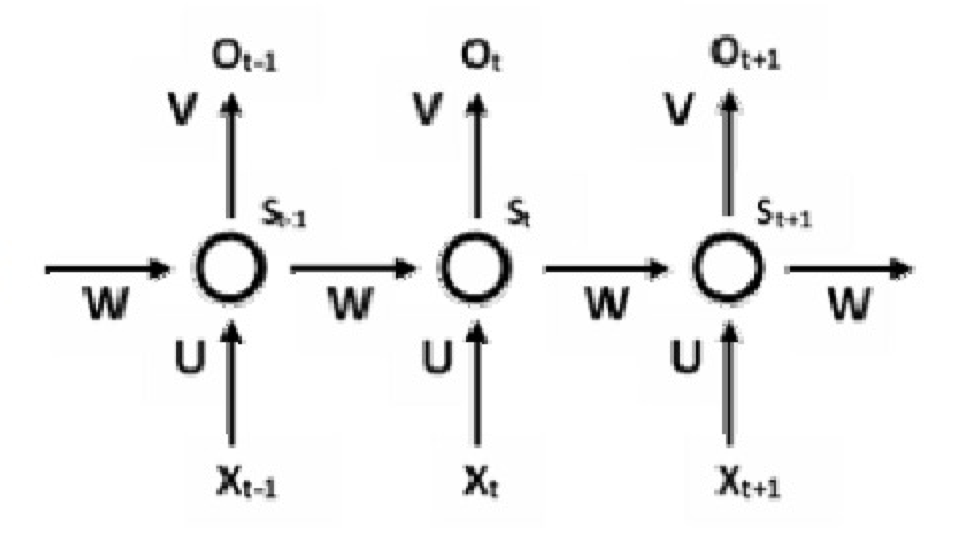
\includegraphics[width=0.6\textwidth]{figures/rnn_net.png}
  \caption{循环神经网络结构}
  \label{fig:rnn}
\end{figure}
\fi %注释结束

\subsection{长短期记忆网络}
从主体上看,LSTM与RNN类似,都是循环神经网络这样的链式结构。而在神经元上看,LSTM细胞节点要比普通的RNN节点要复杂一些。LSTM改进后的神经元由四个不同的神经网络层进行信息的交互,如图~\ref{fig:lstmc}所示。

\begin{figure}[!htb]
  \centering
  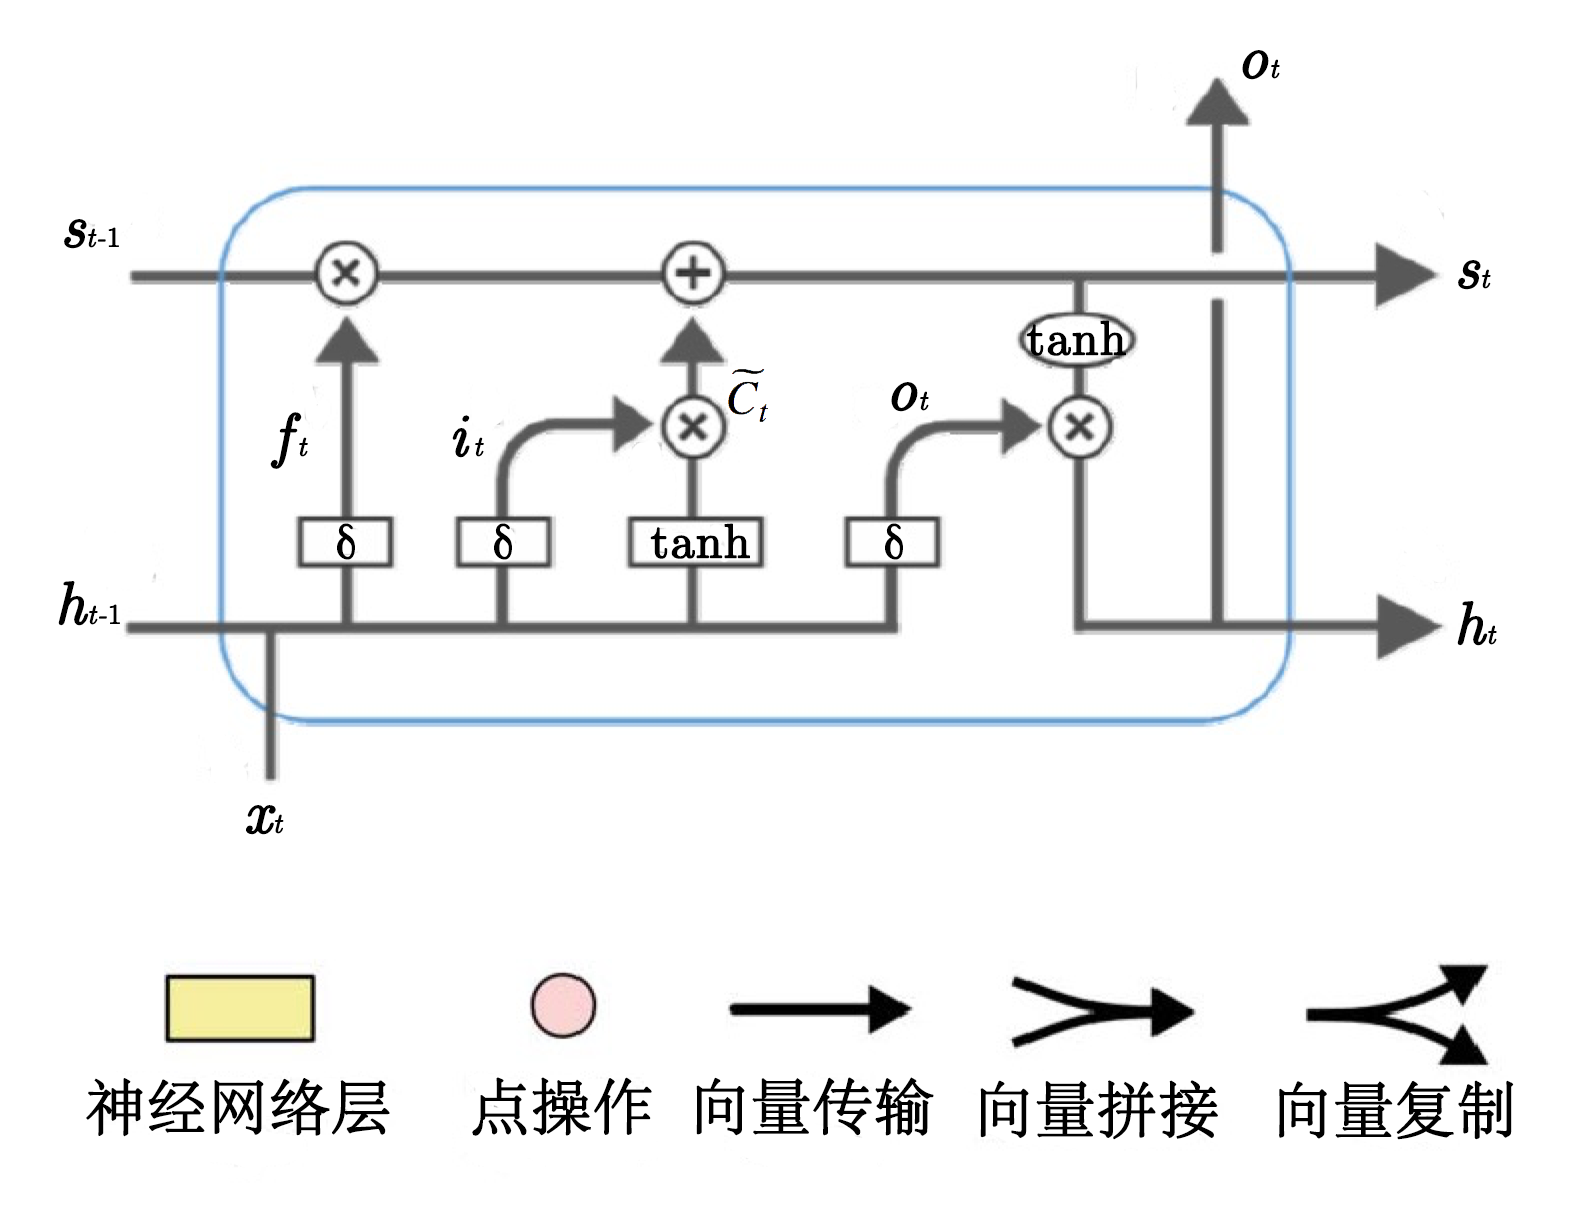
\includegraphics[width=0.6\textwidth]{figures/lstmc.png}
  \caption{LSTM神经元细胞结构图}
  \label{fig:lstmc}
\end{figure}
\hspace{-2em}其中圆形代表基本操作,矩形代表学习得到的状态,箭头代表数据的传输,而箭头的分裂与合并则代表向量的拆分与连接;$s$代表状态,$x$代表输入,$h$代表输出。

在图~\ref{fig:lstmc}中的上方长线段代表了神经网络的状态$s$,它在每个时刻的操作仅在两个地方与输入数据有交互,这就保证了$s$的变化不大,神经元状态比较稳定。LSTM神经元的数据更新由“门”来进行,三个门分别是输入门、遗忘门和输出门,LSTM神经元由此实现数据的更新和储存。

门上的行为由一个点乘Pointwise操作和一个激活函数\textit{Sigmoid}所组成。特别说明,激活函数\textit{Sigmoid}的取值为0至1,分别代表着允许部分信息通过——其中0代表不允许任何信息通过,1代表着允许所有信息通过。

具体的门信息传递机制由以下几个部分完成:
\begin{enumerate}[fullwidth,itemindent=2em,label=\arabic*.]
  %\setlength{\parindent}{4em}
  \item 遗忘门:决定历史信息的保留与遗忘。通过$Sigmoid$函数来决定状态$S$的遗忘程度。
  \begin{equation}
    f_t=\sigma(W_f[h_{t-1}, x_t]+b_f)
    \label{forget}
  \end{equation}
  \item 输入门:决定存储到细胞状态内的新信息。先用$Sigmoid$函数决定记忆的更新程度,然后决定更新的内容,最后将更新的内容加在遗忘内容之上,形成当前时刻的状态。
  \begin{equation}
    \begin{split}
      i_t=\sigma(W_i[h_{t-1}, x_t]+b_i)\hspace{0.2em}\\
      \widetilde{C_t}=\tanh(W_c[h_{t-1}, x_t]+b_c)\hspace{-0.7em}\\
      S_t = f_t·S_{t-1} + i_t · \widetilde{C_t}\hspace{1.1em}
    \end{split}
    \label{input}
  \end{equation}
  \item 输出门:决定输出的值。首先用\textit{Sigmoid}函数决定从状态中输出的部分,然后用$\tanh$对细胞状态进行处理,并与\textit{Sigmoid}函数值相乘,实现输出想输出的部分。
  \begin{equation}
    \begin{split}
      o_t = \sigma(W_o[h_{t-1}, x_t] + b_o)\\
      h_t = o_t*\tanh(S_t)\hspace{1.2em}
    \end{split}
    \label{output}
  \end{equation}
\end{enumerate}
式中,\textit{Sigmoid}函数由模型具体决定,而形如$[\textbf{a}, \textbf{b}]$的操作,代表对两个向量进行拼接(concatenation)。

通过这三个门对神经元的共同作用,LSTM可以完成神经元的基本状态变换,从而完成较好的训练效果。

\section{文本翻译图片相关工作}
文本翻译图片技术中比较原始的模型是CGAN模型\upcite{mirza2014conditional},另一个转折点是Zhang\upcite{zhang2017stackgan}提出的StackGAN模型。本部分将详细阐述GAN的基本原理和在图片生成领域应用的发展历程。

\subsection{GAN模型基本原理}
GANs的基本结构即由一个生成模型$G$和一个判别模型$D$组成。生成模型$G$的目的是尽可能最小化生成与真实训练样本和生成样本的区别,而判别模型$D$的目的则是尽可能最大化地找出真实样本和生成样本之间的区别。

通过多轮迭代生成模型$G$和判别模型$D$的对抗,可以使两个模型都达到上述的目标效果。当训练判别模型$D$的时候,希望输入真实样本$x$可以使判别器对其的判断$D(x)$尽量趋于1,而生成样本$G(x)$通过判别器$D$的时候可以使得$D(G(x))$尽量趋于0。在训练生成模型$G$的时候,输入噪声$z$,希望生成的生成样本通过判别器$D$的时候尽量使得$D(G(z))$趋于0。

可以用简单的数学变换得到公式\eqref{eq:1.1},来描述训练过程。
\begin{equation}
    \label{eq:1.1}
    \min_{G}\max_{D} V_{G,D} = \mathbb{E}_{x \sim P_{data}(x)}[\lg D(x)] + \mathbb{E}_{z \sim P_{G}(z)}[\lg (1-D(G(z)))]
\end{equation}
其中$P_{data}(x)$为真实图片集的分布。

当多轮博弈过后,极大极小问题达到最优解,即纳什均衡,当且仅当$P_z = P_{data}$时\upcite{goodfellow2014generative}。这时$\mathbb{E} D(G(z))$趋于$\frac{1}{2}$,即相当于只能随机猜测0与1,而生成模型$G$学会了真实样本的特性。

相对于传统的生成模型,可以发现GANs模型并不需要使用马尔可夫链,学习过程不需要近似推理,也不需要预先训练,自由度比较高,可以利用反向传播计算梯度,很好地利用了分段线性单元的优势,而可以回避近似计算的困难概率问题。
\subsection{基础GAN模型的缺陷}
GANs模型的缺点对应着优点,比较明显。由于GANs模型自由度太高,在面对过于清晰的图片等训练样本时,收敛性表现较差,生成模型可能出现退化,重复生成相同样本点,导致判别器无法工作,进而导致模型崩溃。因此,在训练过程中,调整好两个模型网络的平衡与同步非常重要。

正因为基础的GAN模型有着这诸多的缺点,所以要选取比较合适的优化GAN模型来生成图片。

\begin{figure}[!htbp]
    \centering
    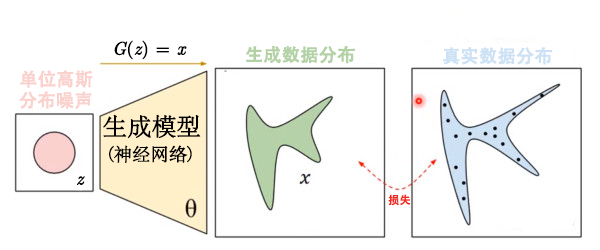
\includegraphics[width=0.8\textwidth]
    {figures/ganprograss.png}\\
    \caption{一般GAN网络模型结构}
    \label{fig:GAN}
  \end{figure}

\subsection{衍生模型分类与特点}
目前对抗生成网络的衍生模型众多,其优化方式大抵由两个大方向衍生而来。一个方向是由损失函数的改变来优化GAN模型的效果,另一个方向则是从模型使用的角度来优化GAN模型的效果。在表~\ref{tab:1.1}中,列举了一些最为常见的GAN模型衍生模型。

\begin{table}[!htb]
    \centering
    \caption{}
    \label{tab:1.1}
    \begin{tabular}{cccc}
        \toprule
        从损失函数角度&\multicolumn{3}{c}{从模型应用角度提出的优化GAN模型}\\
        \cline{2-4}
        提出的优化GAN模型\upcite{fgans}&网络构架角度\upcite{mirza2014conditional}&编码器角度&其他角度改进\\
        \hline
        \multirow{5}{0.3\textwidth}{Least Square GANs, Loss-Sensitive GAN, Fisher GAN, WGAN, WGAN-GP, WGAN-LP, f-GANs\upcite, DRAGAN等}&\multirow{5}{0.19\textwidth}{CGAN, DCGAN, InfoGAN, StackGAN\upcite{zhang2017stackgan}, AL-GAN等}&\multirow{5}{0.19\textwidth}{BEGAN, VAE-GAN, tDCGAN, BiGAN,文献中的算法\upcite{编码器GAN1, 编码器GAN3, 编码器GAN2}等}&\multirow{5}{0.19\textwidth}{LAPGAN, ESRGAN, SRGAN, 3D-GAN, MGAN等}\\ \\ \\ \\ \\
        \bottomrule
    \end{tabular}
\end{table}

图像生成的模型与基于网络构架优化的GAN网络模型最为贴合,本文设计使用StackGAN作为基础,并针对相关实现进行优化。

\subsection{StackGAN及其衍生模型}
Han Zhang et al.在2017年提出了StackGAN模型,创新性地提出了基于栈的对抗式生成网络模型从文本生成图片的方法。

StackGAN和CGAN同属于优化了GAN网络的构架结构的一类GAN模型的分支。其中,StackGAN是对相对朴素的CGAN模型的优化。

\subsubsection{从CGAN到StackGAN}
条件对抗生成网络(Conditional GAN, CGAN)是Mirza\upcite{mirza2014conditional}于2014年提出的,如公式\eqref{eq:CGAN}表述,对生成模型和判别模型输入文本信息作为条件,使用了一个隐藏层的全联通网络(MLP)结构,实现了通过文字标签生成图像的功能。
\begin{equation}
  \min_G\max_DV(G,D)=\mathbb{E}_{x\sim P_{data(x)}}[\lg D(x_i\mid y)]+\mathbb{E}_{x\sim P_G(z)}\lg [(1−D(G(z_i\mid y)))]
  \label{eq:CGAN}
\end{equation}

\begin{figure}[t]
  \centering
  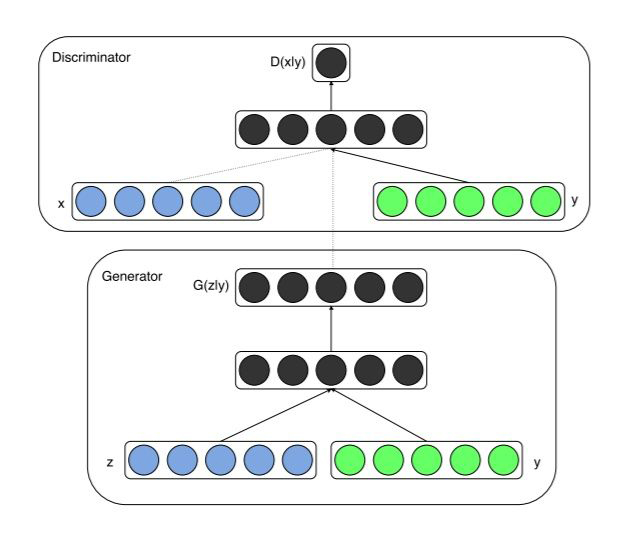
\includegraphics[width=0.5\textwidth]{figures/cgan.jpg}\\
  \caption{CGAN构架示意\upcite{mirza2014conditional}}
  \label{fig:CGAN}
\end{figure}

\begin{figure*}[t] 
  \centering 
  \begin{minipage}[c]{0.6\textwidth} 
    \begin{minipage}[c]{0.9\textwidth}
      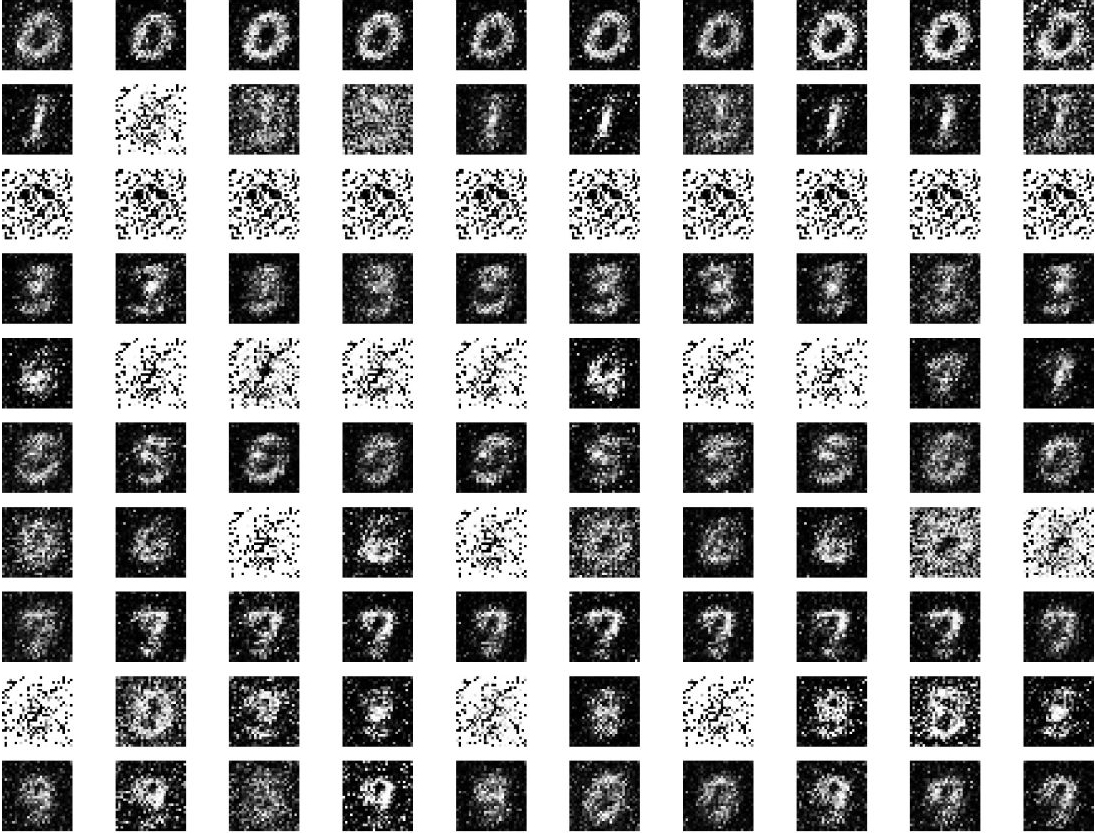
\includegraphics[width=0.45\textwidth]{figures/cgan手写数字1.jpg}\hspace{0.5em}
      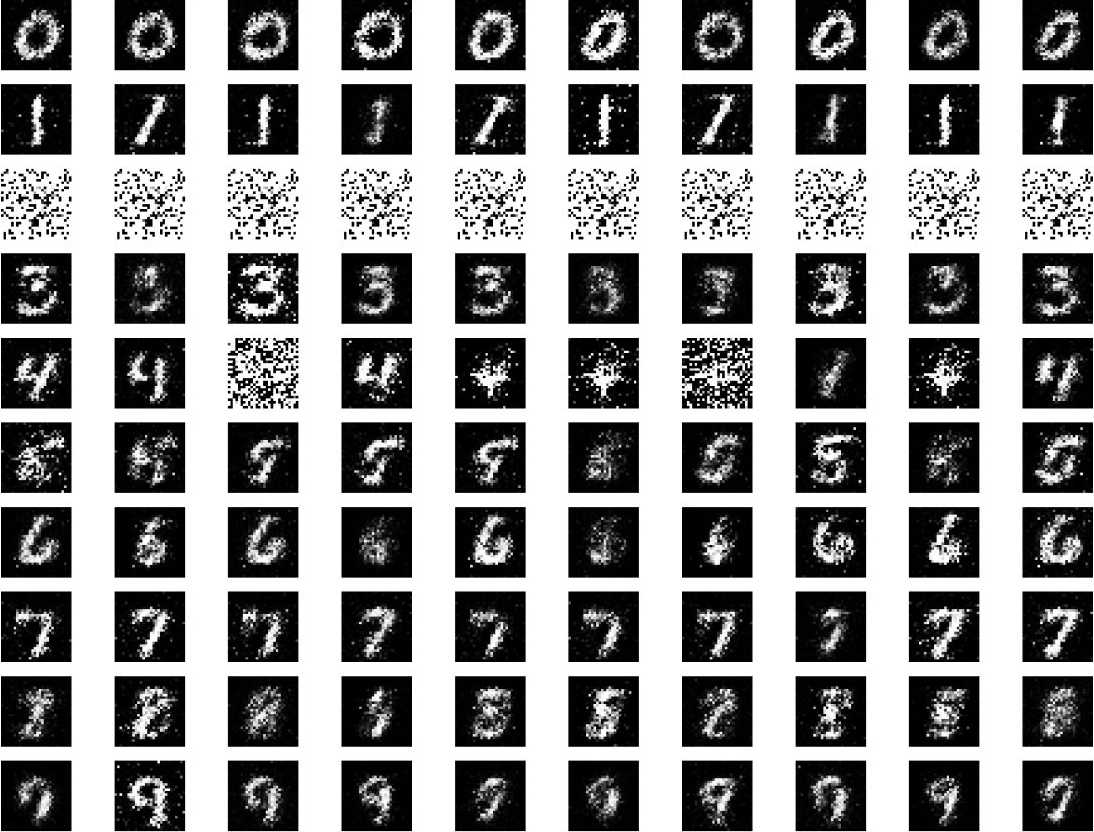
\includegraphics[width=0.45\textwidth]{figures/cgan手写数字2.jpg}
    \end{minipage} 
    \hfill \\ \vspace{0.5em}\\
    \begin{minipage}[c]{0.9\textwidth}
      \hspace{0.22em}
      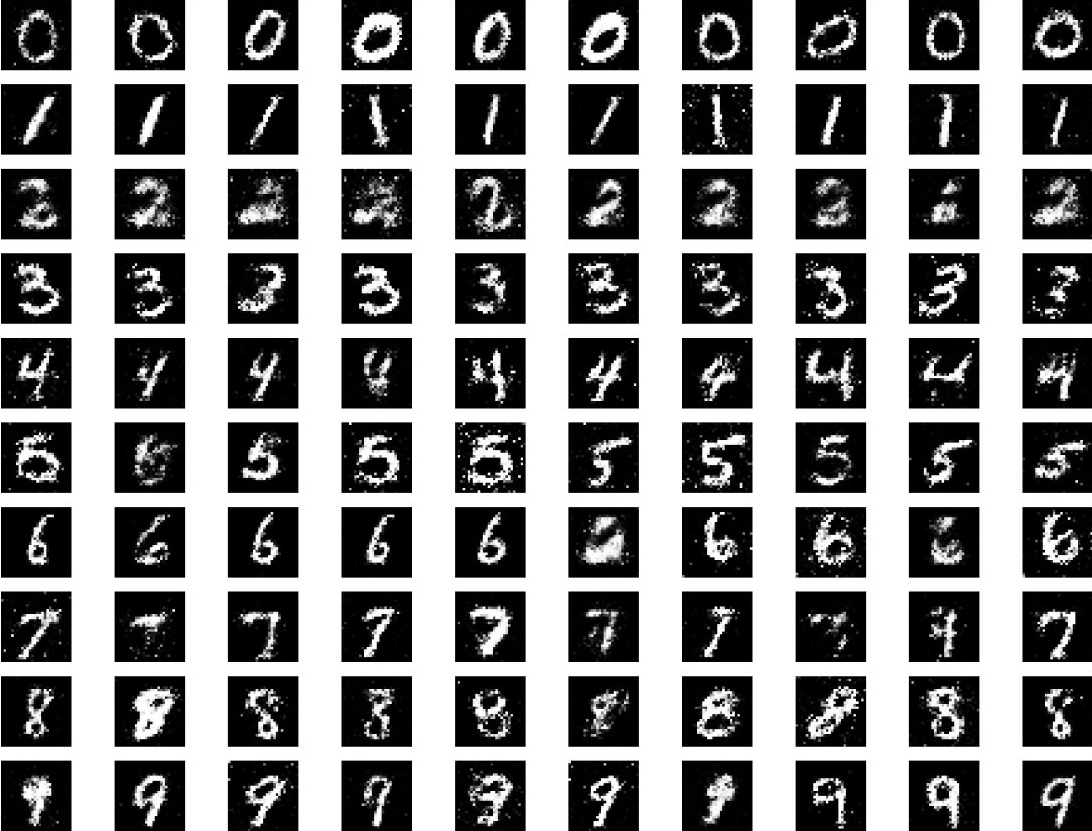
\includegraphics[width=0.45\textwidth]{figures/cgan手写数字3.jpg}\hspace{0.5em}
      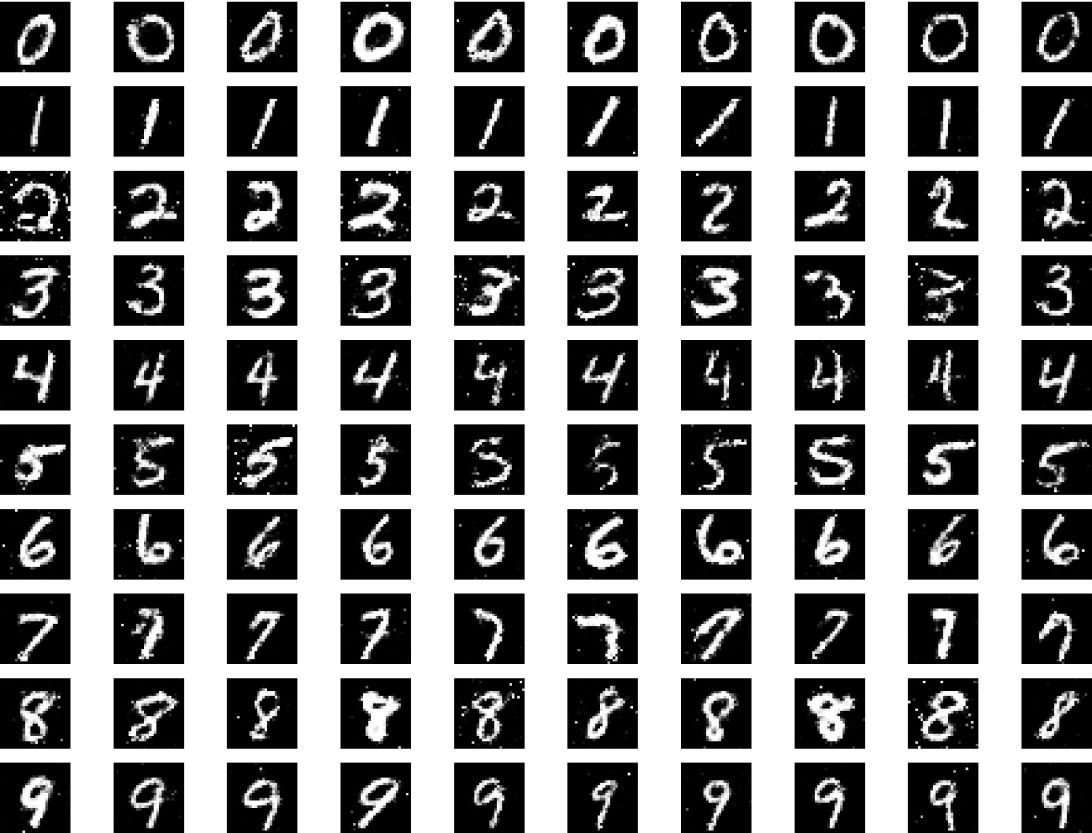
\includegraphics[width=0.45\textwidth]{figures/cgan手写数字.jpg}
    \end{minipage}
  \caption{CGAN生成手写数字\upcite{mirza2014conditional}(分别经历1、10、100、1000 个epoch后的结果)} %,zhihucgan
  \label{fig:cgan手写数字} 
  \end{minipage}
  \hfill 
  \begin{minipage}[c]{0.3\textwidth} 
  \centering%该小页居中排放图片 
  %\vspace{2em}
  \centerline{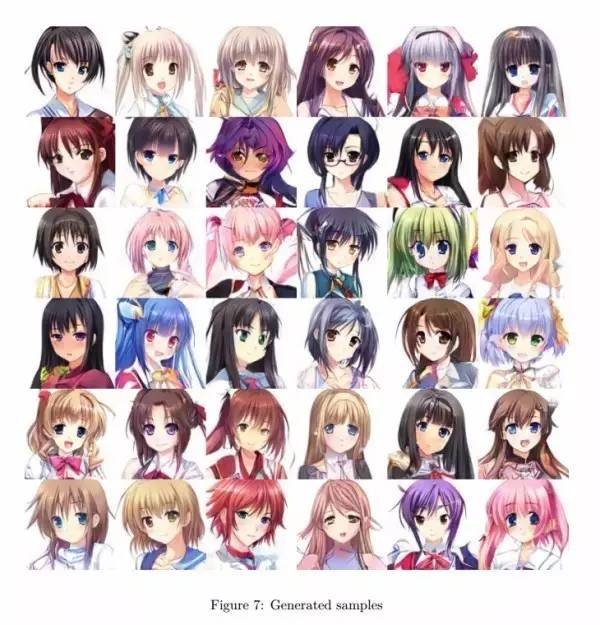
\includegraphics[width=1\textwidth]{figures/moegirl.jpg}}
  %\vspace{2em}
  \caption{CGAN生成二次元头像\upcite{2017comike}} 
  \label{fig:萌娘} 
  \end{minipage} 
  \end{figure*}

但是,CGAN的模型结构简单,效果差,收敛速度慢。在CGAN中,将文本作为条件输入生成器和判别器来训练两个模型生成和判别图像。如图~\ref{fig:cgan手写数字}和图~\ref{fig:萌娘}所示,及时CGAN应用广且有趣,但图像较小,质量不高。最基础的CGAN算法只能生成$64\times64$像素的图片,经过后来的改进,也只能将图片质量提升到$128\times128$像素。

  为了解决这一问题,Han Zhang\upcite{zhang2017stackgan}在2016年提出了StackGAN模型,使用基于栈的结构,分两步进行训练。
  
  如图~\ref{fig:StackGAN}所示,第一步先训练模型使模型生成$64\times 64$像素的图片,训练出的模型只能输出像素低、形状有所扭曲的图片。第一次训练的时候并不使用转化为向量的文字直接作为输入,因为这一向量为1024维,过于稀疏,不利于深度的训练。在经历一次FC以后进行输入,这样可以增强表现。
  第一阶段训练的损失函数为式\eqref{stackgan_loss1}所示。
  第二次训练并不增加噪声输入,经过多轮残差网络迭代,
  %残差网络可以实现梯度的跨层传播,解决深度网络里面梯度消失的问题
  模型修正一轮训练生成图片的错误,并且在图像中添加细节,生成$256\times256$像素的“高清图片”。
  第二阶段训练的损失函数如式\eqref{stackgan_loss2}所示。
  \begin{equation}
    \begin{aligned}
      &&\mathcal{L}_{D_0} = & \mathbb{E}_{(I_0,t) \sim P_{data}}[\lg D_0 (I_0,\varphi_t)] \\ && &+\mathbb{E}_{z\sim P_z,t \sim P_{data}}[\lg (1-D_0(G_0(z, \hat{c}_0 ),\varphi_t))],
      \\
      &&\mathcal{L}_{G_0} = & \mathbb{E}_{z\sim P_z,t \sim P_{data}}[\lg (1-D_0(G_0(z, \hat{c}_0 ),\varphi_t))]  \\ && &+\lambda D_{KL}(\mathcal{N}(\mu_0(\varphi_t),\Sigma_0(\varphi_t))\parallel \mathcal{N}(0,I))
      \end{aligned}
    \label{stackgan_loss1}
  \end{equation}
  \begin{equation}
    \begin{aligned}
      &&\mathcal{L}_{D} = & \mathbb{E}_{(I,t) \sim P_{data}}[\lg D (I,\varphi_t)] \\ && &+\mathbb{E}_{s_0\sim P_{G_0},t \sim P_{data}}[\lg (1-D(G(s_0, \hat{c} ),\varphi_t))],
      \\
      &&\mathcal{L}_{G} = & \mathbb{E}_{s_0\sim P_{G_0},t \sim P_{data}}[\lg (1-D(G(s_0, \hat{c} ),\varphi_t))]  \\ && &+\lambda D_{KL}(\mathcal{N}(\mu(\varphi_t),\Sigma(\varphi_t))\parallel \mathcal{N}(0,I))
      \end{aligned}
    \label{stackgan_loss2}
  \end{equation}
    
  \begin{figure}[!htb]
    \centering
    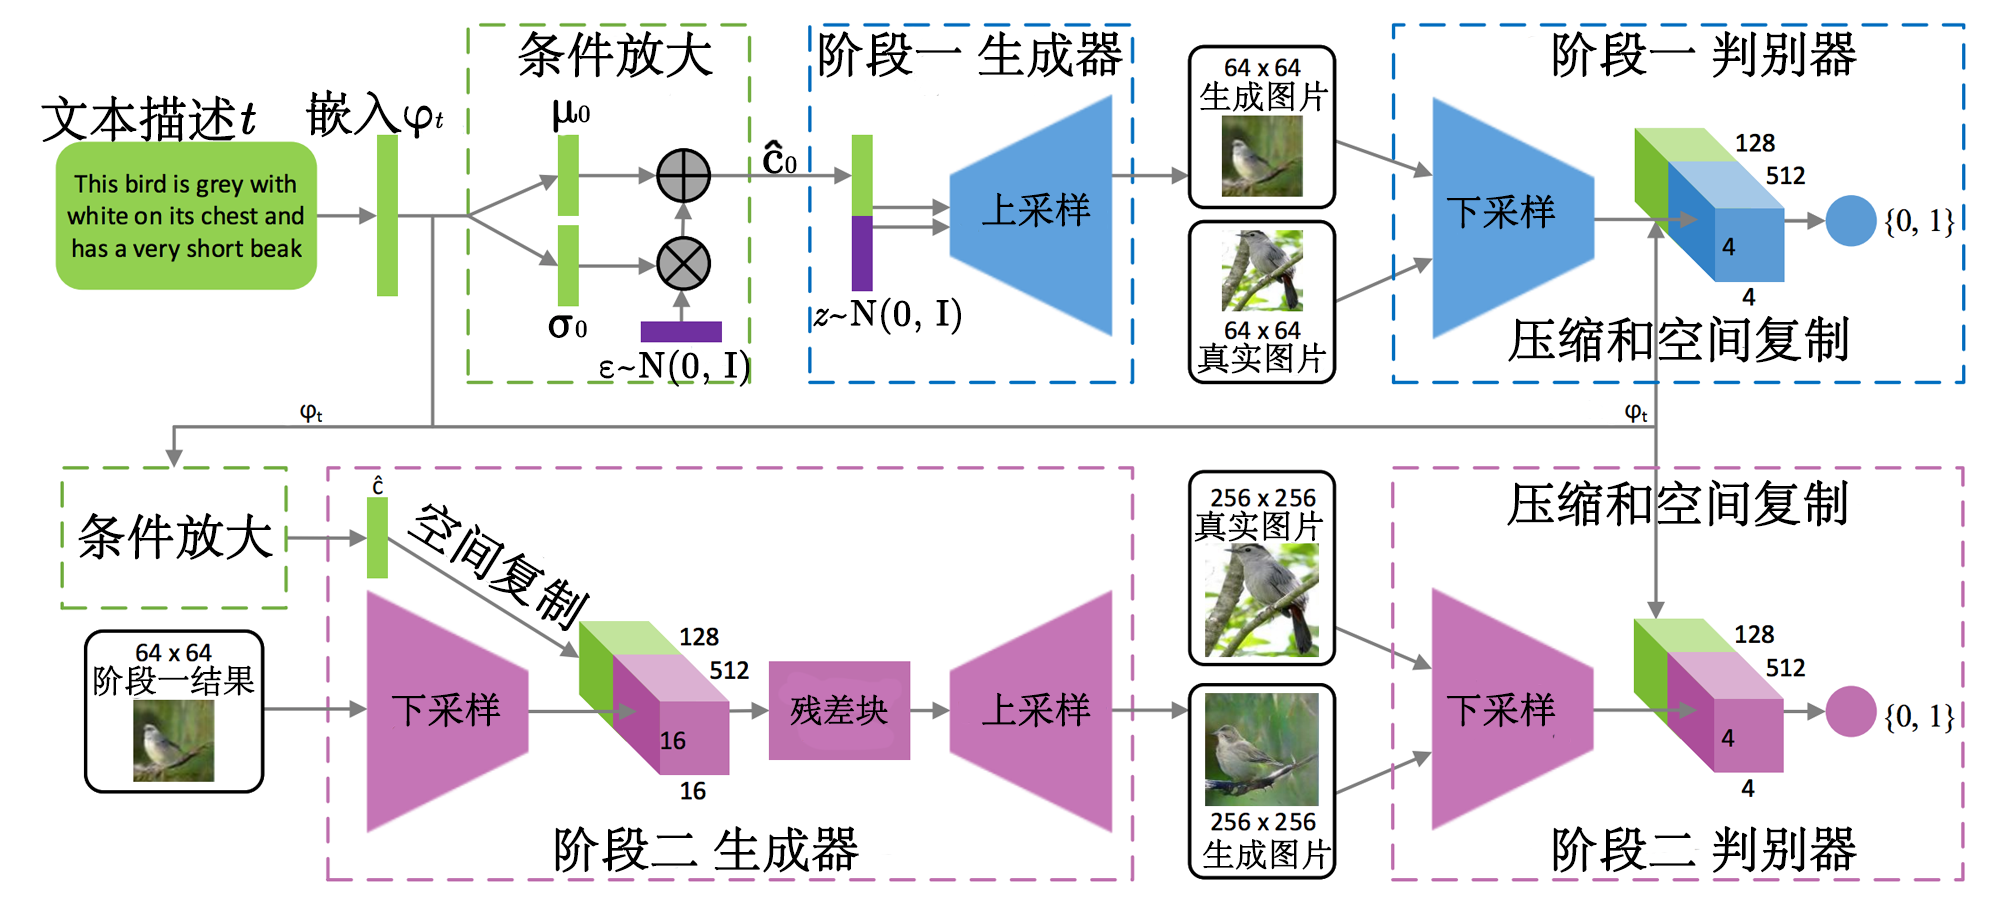
\includegraphics[width=0.95\textwidth]{figures/StackGAN.png}\\
    \caption{StackGAN构架示意}
    \label{fig:StackGAN}
  \end{figure}


  StackGAN模型相比较于CGAN模型,可以生成更高清的图片,而且结构更为真实。

\subsubsection{对StackGAN的进一步优化与运用}
同一课题组紧接着提出了StackGAN++\upcite{zhang2018stackgan++},对原有算法进一步进行了优化。StackGAN++模型也叫做StackGAN\_v2,对之前的StackGAN模型主要有三点改进。第一,改为采取树状结构作为输入,通过不同的生成器来生成不同尺寸的图片,多层次叠加形成了有位置关系的“假图片”,即混合图层叠加图片;第二,额外引入了非条件性的损失,直接将服从正态分布的损失$z$叠加在最后生成的“假图片”上;第三,引入了色彩限制,限制了最终“假图片”的色彩信息分布。

李飞飞课题组的Johnson\upcite{Johnson_2018}在StackGAN模型之上,提出了自己的优化。

该方法主要有三个特点:第一是有一个处理场景图的方法,第二是确保了生成的图像中个物体正确,且位置关系合理。第三是确保了生成图像的质量比较好。
其具体技术路线将在下一章进行推导和研究。

\section{本章小结}
本章主要总结了本次技术方案的前置技术,包括神经网络中的LSTM-RNN长短期记忆循环神经网络模型和StackGAN模型及其相关技术。LSTM-RNN模型是一种相对稳定、收敛,可以一定程度上避免梯度消失的深度学习模型,主要为下一章实现图片标注方法的技术做好铺垫。StackGAN及其升级版本是Han Zhang及其他科研人员2016年其后提出的一系列理论,本章内简要阐释了它的背景、原理和与后续技术的比较,决定使用李飞飞课题组的场景图像生成方法作为实现的理论依据,也为下一章自然语言生成图片的方法做好了前置说明。